\documentclass[conference]{IEEEtran}
\usepackage{cite}
\usepackage{amsmath,amssymb,amsfonts}
\usepackage{algorithmic}
\usepackage{graphicx}
\usepackage{textcomp}
\usepackage{xcolor}
\usepackage{float}
\usepackage{booktabs}
\usepackage{url}
\usepackage{siunitx}

\def\BibTeX{{\rm B\kern-.05em{\sc i\kern-.025em b}\kern-.08em
    T\kern-.1667em\lower.7ex\hbox{E}\kern-.125emX}}

\begin{document}

\title{ML441 Assignment 3}

\author{\IEEEauthorblockN{RH Buhr, 26440873}
\IEEEauthorblockA{\textit{BDatSci Programme, 4th Year} \\
\textit{Stellenbosch University}\\
Stellenbosch, South Africa \\
26440873@sun.ac.za}
}

\maketitle

\begin{abstract}

\end{abstract}

\section{\textbf{Introduction}}

\section{\textbf{Background}}

\subsection{\textbf{Recurrent Neural Networks}}

Recurrent Neural Neworks are a type of neural network specifically designed to handle sequential data, where there exists temporal dependencies between observations. RNNs incorporate feedback connections that allow information from prior steps to influence future predictions, which is what makes them well-suited for time series data, such as language translation, natural language processing, sentiment analysis, speech recognition, image captioning, etc.

RNNs extend traditional neural networks by incorporating a hidden state that carries information from one time step to the next. This creates a feedback loop, allowing the network to retain context from previous time steps and use it to influence the current time step. At each time step, the RNN processes the new input together with the hidden state from the previous time step, which allows the model to capture temporal dependencies in time series data. Unlike traditional neural networks, like feedforward neural networks, RNNs share hyperparameters across time steps and are trained using backpropagation through time, as opposed to regular backpropagation \cite{ibm_rnn}.

\begin{figure}[H]
  \centering
  \includegraphics[width=0.65\linewidth]{images/ibm_rnn.jpg}
  \caption{Rolled and unrolled views of an RNN (\cite{ibm_rnn}).}
  \label{fig:ibm_rnn}
\end{figure}

Figure~\ref{fig:ibm_rnn} shows a rolled RNN with its unrolled counterpart which has been unrolled over time. Each time step takes $X_t$ and the previous hidden state as input, produces and output $Y_t$ and passes the hidden state to the next time step.

\subsubsection{\textbf{Elman RNN}}

The Elman RNN is considered the vanilla RNN. Its defining factor is the hidden state that stores information from the previous time steps and passes it along to the next time step.

Formally, the Elman RNN is defined as:

$$
h_t = \sigma_h(W_x x_t + W_h h_{t-1} + b_h)
$$

$$
y_t = \sigma_y(W_y h_t + b_y)
$$

where:

\begin{itemize}
    \item $x_t$ is the input vector at time step t.
    \item $y_t$ is the output vector at time step t.
    \item $h_t$ is the hidden state at time step t.
    \item $W_x$ is the input weight matrix.
    \item $W_h$ is the recurrent weight matrix.
    \item $W_y$ is the output weight matrix.
    \item $b_h$ is the hidden state bias term.
    \item $b_y$ is the output bias term.
    \item $\sigma_h$ is a non-linear activation function (e.g. ReLu, sigmoid, tanh).
    \item $\sigma_y$ is an activation function suited for the machine learning task at hand (e.g. softmax for multi-class classification).
\end{itemize}

The inclusion of $W_h h_{t-1}$ in the hidden state of Elman RNNs distinguishes them from traditional models and allows them to maintain memory of past context \cite{elman_rnn}.

\subsubsection{\textbf{Jordan RNN}}

Unlike the Elman RNN, where the hidden state depends on the previous hidden states, the Jordan RNN hidden state depends on previous outputs. This allows the Jordan RNN to integrate information from its own past predictions when updating the current hidden layer.

Formally, the Jordan RNN is defined as:

$$
h_t = \sigma_h(W_x x_t + W_h y_{t-1} + b_h)
$$

$$
y_t = \sigma_y(W_y h_t + b_y)
$$

The use of $W_h y_{t-1}$ in the hidden state instead of $W_h h_{t-1}$ is what sets Jordan RNNs apart from Elman RNNs. This means Jordan RNNs capture sequential information differently than Elman RNNs, which can make them more efficient in settings where the model's own predictions strongly influence the outcome of the current and future time steps \cite{jordan_rnn}.

\subsubsection{\textbf{Multi-RNN}}

Multi-RNNs can be thought of as a combination between Elman and Jordan RNNs by incorporating feedback from both the previous hidden state and the previous output. This allows Multi-RNNs to model sequential information more flexibly, since the current hidden representation does not only depend on the internal memory of the network but also its previous predictions.

The Multi-RNN can be expressed as:

$$
h_t = \sigma_h(W_x x_t + W_hh y_{t-1} + W_hy y_{t-1} + b_h)
$$

$$
y_t = \sigma_y(W_y h_t + b_y)
$$

The difference is captured in the inclusion of $W_hh y_{t-1} + W_hy y_{t-1}$ in the hidden state allowing Multi-RNNs to capture richer temporal information.

\subsubsection{\textbf{RNN Limitations}}

While RNNs are powerful tools for time series problems, they suffer from critical limitations, especially when faced with long sequences. The main issue under consideration is known as the Vanishing/Exploding Gradient Problem. During backpropagation through time, gradients can either shrink to near zero or grow excessively. This makes it difficult for the network to capture long-term dependencies and can lead to unstable learning. As a result, RNNs often struggle when context from distant time steps is needed to accurately predict the current time step. Mitigations include, gradient clipping, selection of problem appropriate activation functions, better weight initialization, learning rate control, and the use of more advanced architectures like LSTM \cite{rnn_problems}. 
\subsection{\textbf{Datasets}}

The recurrent neural networks were trained and evaluated across five distinct datasets to provide a comprehensive assessment of their performance across diverse tasks.

\subsubsection{\textbf{AMD Stock Data}}

The AMD dataset records AMD (Advanced Micro Devices) stock data over a period of 40 years. The dataset records 10098 instances of 7 variables:

\begin{itemize}
    \item \texttt{Date}: Date the instance was recorded in the format 'yyyy-mm-dd'.
    \item \texttt{Open}: The price at which the stock first traded on the trading day.
    \item \texttt{High}: The highest price the stock reached during the trading day.
    \item \texttt{Low}: The lowest price the stock reached during the trading day.
    \item \texttt{Close}: The final price of the stock when the market closed on that day.
    \item \texttt{Adj Close}: The closing price adjusted for corporate actions like stock splits or dividends.
    \item \texttt{Volume}: The total number of shares traded on that day.
\end{itemize}

This is a regression problem, with \texttt{Adj Close} as the response, instead of \texttt{Close}, because it reflects the true economic value of the stock by incorporating adjustments, these adjustments ensure the data more accurately reflects the stock market trends.

\begin{figure}[H]
    \centering
    \includegraphics[width=0.5\textwidth]{images/amd_adj_close.pdf}
    \caption{AMD Adjusted Closing Prices Over Time}
    \label{fig:amd_adj_close}
\end{figure}

Figure~\ref{fig:amd_adj_close} displays how AMD's adjusted closing price fluctuated from 1980 through 2020. The series is clearly non-stationary, with periods of sharp growth and declines. The overall trend is upward, even though there are multiple crashes. Most notably around the early 2000s dot-com bubble and the 2008 financial crisis. The defining upward trend, showing rapid growth, started in 2020.

To formally asses stationarity, and Augmented Dickey-Fuller (ADF) test was conducted. The ADF test is a widely used statistical procedure for detecting unit roots in time series data. If a series has a unit root, it means it behaves like a random walk and is thus non-stationary. The ADF statistic of the AMD stock dataset yielded a p-value of 0.05468, meaning the null hypothesis is not rejected at the 5\% significance level and the series is non-stationary.

The series also exhibits no clear periodic seasonal structure, which is visually evident. Overall the dataset demonstrates the characteristics of a typical non-stationary financial time series, with long-term upward trend, \cite{stock_market_dataset_amd}.

\subsubsection{\textbf{Air Quality}}

The Air Quality dataset records hourly averaged responses of a gas multi-sensor device deployed in an Italian city between March 2004 to February 2005. The dataset records 9358 instances with multiple variables including pollutants ($CO$, $NMHC$, $C_6H_6$, $NO_x$, $NO_2$), sensor responses from five metal oxide sensors,as well as temperature, relative humidity, and absolute humidity.

For this study the focus is on \texttt{CO(GT)}, concentration of carbon monoxide in $mg/m^3$, making this a regression problem.

\begin{figure}[H]
\centering
\includegraphics[width=0.5\textwidth]{images/air_q_over_time.pdf}
\caption{Air Quality Over Time: CO(GT) with 24h and 7d rolling means}
\label{fig:air_q_over_time}
\end{figure}

Figure~\ref{fig:air_q_over_time} shows the hourly CO(GT) values along with 24-hour and 7-day rolling averages. The raw series is highly volatile, with frequent spikes while the rolling means reveal drifts in the $CO$ concentration. These shifts indicate that although the hourly data are noisy, there are underlying patterns driven by human activity and environmental causes.

The dataset is missing some pollutant measurement entries, recorded as placeholder value \textbf{-200}, this leads to visible gaps in the series.

\begin{figure}[H]
\centering
\includegraphics[width=0.5\textwidth]{images/air_q_seasonal.pdf}
\caption{Seasonal decomposition of CO(GT) series}
\label{fig:air_q_seasonal}
\end{figure}

Figure~\ref{fig:air_q_seasonal} shows the seasonal decomposition of the \texttt{CO(GT)} series. The trend component highlights longer-term fluctuations, where the average $CO$ levels decrease during mid 2004 and increase again toward late 2004 and early 2005. The seasonal component reveals clear short-term periods, consistent with daily and weekly cycles, possibly linked to human activity.

To assess stationarity an ADF test was done. The test yielded a p-value of $2.498 \times 10^{-16}$, meaning the null hypothesis of the unit root is rejected and the \texttt{CO(GT)} series can be considered stationary. Although the data exhibits short term cycles and noisy behavior, the statistical properties remain stable over time.

In summary the Air Quality dataset exhibits short-term variability, seasonal cycles and a stationary structure. This makes it a suitable candidate for time series modeling with recurrent neural networks, \cite{air_quality}.

\subsubsection{\textbf{Garment Productivity}}

The Garment Productivity dataset records worker productivity across multiple production units in a garment factory over a three month period. It contains 1197 instances of 15 variables that capture operational metrics and contextual information:

\begin{itemize}
    \item \texttt{date}: The date the observation was make, in the format 'yyyy-mmm-dd'.
    \item \texttt{quarter}: Specifies the portion of the month data was collected.
    \item \texttt{department}: Indicates the department of the instance (\textit{sewing or finishing}).
    \item \texttt{day}: Day of the week.
    \item \texttt{team}: Identifier for the production team.
    \item \texttt{targeted\_productivity}: The management determined productivity target (between 0 and 1).
    \item \texttt{smv}: Standard Minute Value, it is the allocated time for a task.
    \item \texttt{wip}: Work-in-Progress, includes the number of unfinished items in the pipeline.
    \item \texttt{over\_time}: Total over-time work.
    \item \texttt{incentive}: Financial incentive allocated to the team.
    \item \texttt{idle\_time}: Time lost due to miscellaneous reasons.
    \item \texttt{idle\_men}: Number of workers who were idle due to production interruption.
    \item \texttt{no\_of\_style\_change}: Number of times the style being produced was changed.
    \item \texttt{no\_of\_workers}: Number of workers in the team.
    \item \texttt{actual\_productivity}: The actual productivity measure achieved by the workers (also between 0 and 1).
\end{itemize}

This dataset combines continuous variables with categorical variables. This distinguishes it from the above mentioned datasets.

\begin{figure}[H]
\centering
\includegraphics[width=0.5\textwidth]{images/actual_prod.pdf}
\caption{Actual Productivity Over Time}
\label{fig:actual_prod}
\end{figure}

Figure~\ref{fig:actual_prod} shows how the average daily productivity changes over time. The plot indicates that the overall trajectory is relatively stable, with fluctuations driven by workload variation, overtime, etc. There appears to be no seasonal pattern, since the data was recorded over a very small window.

An ADF test was conducted to formally investigate stationarity. The test returned a p-value of 0.001457, which is below the 5\% threshold. Thus the garment series is considered stationary, \cite{garment_productivty}.

\subsubsection{\textbf{Room Occupancy}}

The Occupancy dataset records environmental conditions and room occupancy information for an office space. The dataset contains 20560 minute-by-minute measurements of 7 variables:

\begin{itemize}
    \item \texttt{Date}: Timestamp of the measurement, in the format 'yyyy-mm-dd hh:mm:ss'.
    \item \texttt{Temperature}: Ambient temperature of the room (\si{\celsius}).
    \item \texttt{Humidity}: Relative humidity (\%).
    \item \texttt{Light}: Ambient illumination level (Lux).
    \item \texttt{CO2}: Carbon dioxide concentration (ppm).
    \item \texttt{HumidityRatio}: Specific humidity (ratio of water vapor to dry air).
    \item \texttt{Occupancy}: Binary response variable, where 1 indicates the room was occupied and 0 indicates it was vacant.
\end{itemize}

\begin{figure}[H]
\centering
\includegraphics[width=0.5\textwidth]{images/occupancy_over_time.pdf}
\caption{Room Occupancy Over Time}
\label{fig:occupancy_over_time}
\end{figure}

Figure~\ref{fig:occupancy_over_time} shows the occupancy status over time, plotted as the raw binary response series and rolling averages over 60 minutes and 6 hours. The raw occupancy data exhibits abrupt shifts between 0 and 1, reflecting sudden transitions as people enter the room and leave it vacant again. The rolling averages reveal broader trends, the 60-minute window smooths out short-term fluctuations within hours, while the 6-hour window reveals daily cycles, showing how occupancy changes during working and non-working hours.

To formally assess stationarity an ADF test was conducted on the binary response variable, \texttt{Occupancy}. The \texttt{Occupancy} ADF test resulted in a p-value of $5.08e-09$, which means the series is stationary. This can also be confirmed by looking at the plot in figure~\ref{fig:occupancy_over_time}.

The Occupancy dataset exhibits no clear trend, but shows very strong daily seasonality. As mentioned the office is occupied during the day and vacant during the night, which is a form of 24-hour seasonality, \cite{occupancy_detection}.

\subsubsection{\textbf{Max Planck Institute Weather Data}}

The Weather dataset records meteorological observations at the Max Planck Institute every 10 minutes over the course of one year. The dataset contains 52560 observations of 20 atmospheric variables, which include temperature, air pressure, potential temperature, dew point temperature, relative humidity, vapor pressure measures, specific humidity, water content, air density, wind velocity and direction, as well as radiation and precipitation indicators. 

Temperature (in \si{\celsius}) is the response variable of interest. This dataset thus represents a regression problem where the goal is to forecast the temperature based on other meteorological data.

\begin{figure}[H]
    \centering
    \includegraphics[width=0.5\textwidth]{images/temp_over_time.pdf}
    \caption{Temperature Over Time}
    \label{fig:temp_over_time}
\end{figure}

Figure~\ref{fig:temp_over_time} shows how the observed temperature changed throughout the measurement period. The time series exhibits a seasonal pattern, with temperature increasing from January to July, peaking in the summer months, and then decreasing toward December. This is expected of climactic time series data.

An ADF test was conducted, and yielded a p-value of $2.149e-13$, which is well below the 0.05 significance threshold. This means the series is stationary.

In summary, the dataset provides a comprehensive representation of atmospheric conditions and demonstrates the dynamics of meteorological processes, where the response variable (temperature) is influenced by multiple interacting environmental factors \cite{weather_dataset}.

\subsection{\textbf{RNN Training \& Hyperparameter Tuning}}

Unlike traditional data, time series data contains temporal dependencies between observations. This means that traditional k-fold cross-validation cannot be used to evaluate models trained on time series data. Randomly partitioning a time series into folds can result in information leakage between future and past observations.

A more suitable cross-validation strategy that can be used with time series data and RNNs is cross-validation on a rolling basis.

\begin{figure}[H]
  \centering
  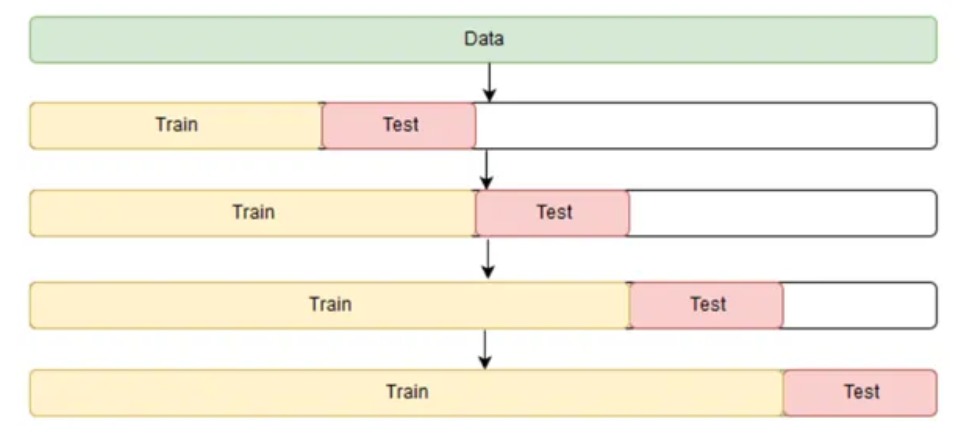
\includegraphics[width=0.65\linewidth]{images/rolling_cv.png}
  \caption{Cross-validation on a Rolling Basis (\cite{time_series_cv}).}
  \label{fig:rolling_cv}
\end{figure}

Figure~\ref{fig:rolling_cv} illustrates the basic idea of cross-validation on a rolling basis. The process starts with a small subset of the data used for training, with the subsequent subset used for testing. The data tested on is then used for the next training set and the subsequent subset is then used for testing. This procedure repeats until the end of the series.

Another approach is blocked cross-validation, where the series is divided into non-overlapping contiguous blocks, each block is used once as a validation set. This method avoids temporal leakage but may be less efficient in utilizing the full dataset compared to rolling schemes \cite{time_series_cv}.

Hyperparameter tuning for RNNs typically involve exploring architectural and training parameters. Important hyperparameter categories and examples include:

\begin{itemize}
    \item \textbf{Network Architecture}: Number of hidden layers, number of neurons per layer, choice of RNN variant.
    \item \textbf{Training Parameters}: Learning rate, optimizer type, batch size, sequence length, gradient clipping thresholds.
    \item \textbf{Regularization}: Dropout probability, weight decay.
\end{itemize}

Strategies such as grid search or random search using cross-validation can be used to explore the hyperparameter space and determine the best combination. The accuracy metric used to evaluate the models during the cross-validation process is entirely problem dependent, e.g. MSE used for regression, and accuracy for classification

\section{\textbf{Implementation}}

\section{\textbf{Empirical process}}

\section{\textbf{Results \& discussion}}

\section{\textbf{Conclusion}}

\bibliographystyle{plain}
\bibliography{references}
\vspace{12pt}

\end{document}
